\documentclass[11pt, a4paper,twocolumn]{jarticle}
\usepackage[dvipdfmx]{graphicx}

\begin{document}
%=============================================================
\section{Learnig Matlab compatible scientific programing language software (Octave) and understanding First Fourier Transform (FFT) of the captured sound waves ($4^{th} day$)}
% ===============================================================
\subsection{Purpose}
今回の実験ではMatlab互換の数値計算ソフトウェアであるGNU Octaveを用いて取り込んだ音声データをフーリエ変換(離散型高速フーリエ変換)することで,周波数分解する.これらの実験を通して,信号のフーリエ変換を理解する.
% =======================================================
\subsection{Procedure}
\noindent
\textbf{Task 4.1} \\
任意の周波数,振幅のSin波およびCos波のフーリエ変換を行い,それぞれ実部,虚部,パワースペクトルを表示する.
この時横軸をHzにすることに注意する.
またこの得られたグラフが何を意味するのかを考える.
今回の実験では振幅1,周波数262HzのCos波Sin波のFFTを行った.

\noindent
\textbf{Task 4.2} \\
Task3.2と同様の方法で音叉(二種類)から音声信号を読み込みデジタル信号を取得する.
この際サンプリング周波数を1kHz,データ数1000として測定を行なった.
今回は330Hzと440Hzの音叉をそれぞれ鳴らした.
その後その時間領域でのデジタル信号をOctaveでフーリエ変換し周波数領域の信号を得る.
得られた周波数領域の信号において330Hz,440Hzの周波数が含まれているのかを調べる.

% =======================================================
\subsection{Result}
\noindent
\textbf{Task 4.1} \\
262Hzの正弦波,余弦波のフーリエ変換の結果を以下に示す.
グラフは上から実部,虚部,パワースペクトルの順で表されている.

\begin{figure}[htbp]
 \begin{center}
  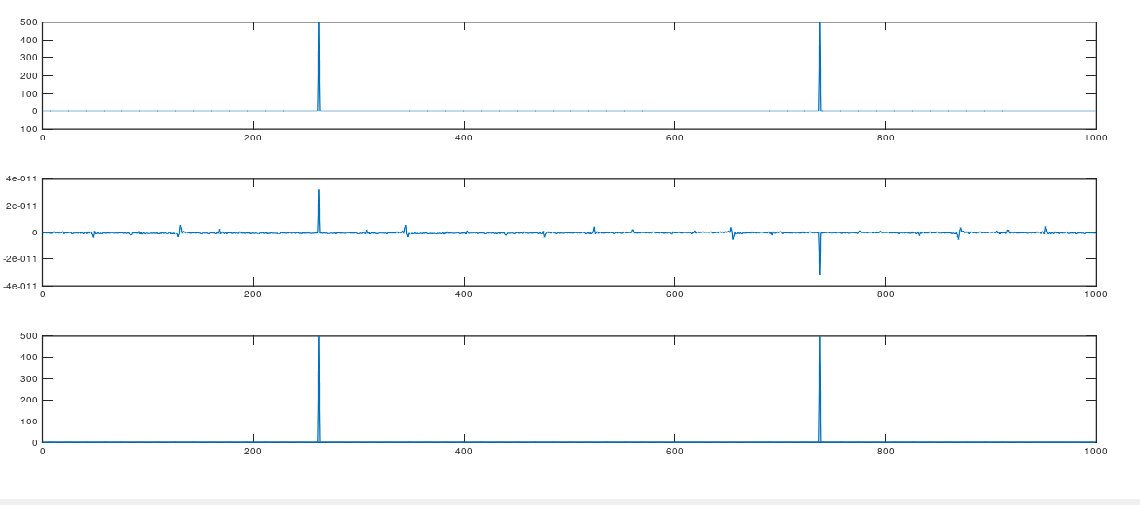
\includegraphics[width=0.8\linewidth]{fig22.png}
 \end{center}
 \caption{262Hz余弦波FFT}
 \label{fig:22}
\end{figure}

\begin{figure}[htbp]
 \begin{center}
  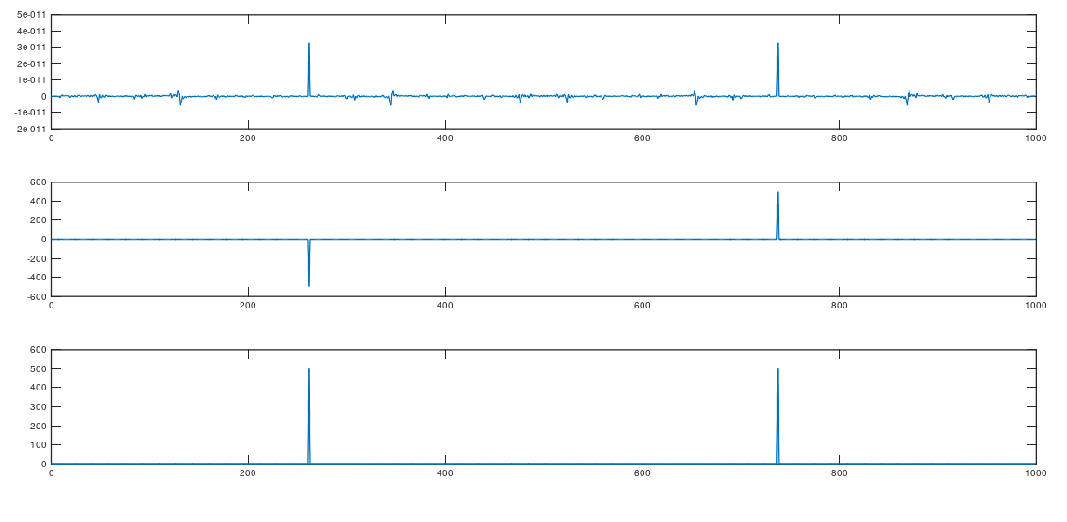
\includegraphics[width=0.8\linewidth]{fig23.png}
 \end{center}
 \caption{262Hz正弦波FFT}
 \label{fig:23}
\end{figure}

\noindent
\textbf{Task 4.2} \\
330Hzと440Hzの音叉をそれぞれ鳴らした際にマイク回路により得られた音波を0V中心に振動するように2.5V引いた時の測定値をプロットしたグラフを図\ref{fig:24},図\ref{fig:26}に示す.
さらにその結果をフーリエ変換した際の周波数領域のグラフを図\ref{fig:25},\ref{fig:27}に示す

\begin{figure}[htbp]
 \begin{center}
  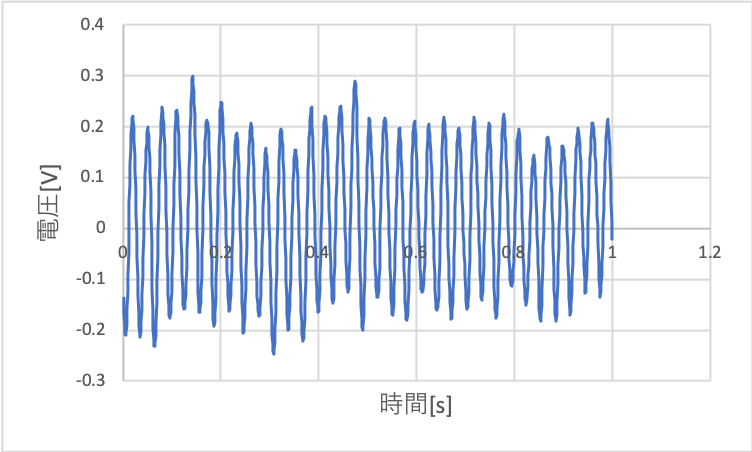
\includegraphics[width=0.8\linewidth]{fig24.png}
 \end{center}
 \caption{330Hz音叉の測定値}
 \label{fig:24}
\end{figure}

\begin{figure}[htbp]
 \begin{center}
  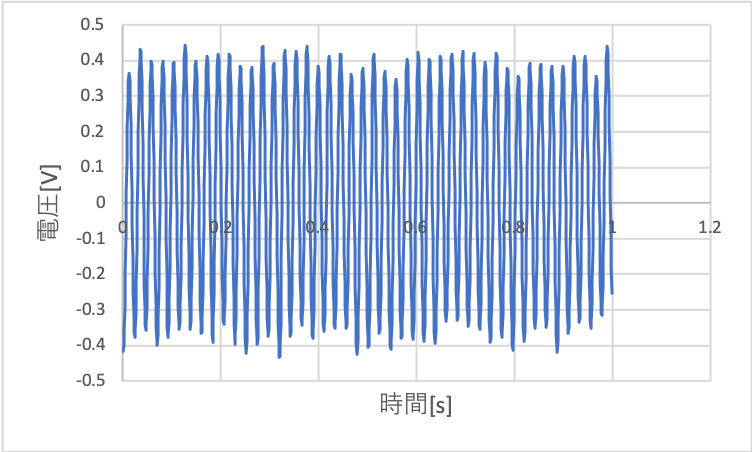
\includegraphics[width=0.8\linewidth]{fig26.png}
 \end{center}
 \caption{440Hz音叉の測定値}
 \label{fig:26}
\end{figure}

\begin{figure}[htbp]
 \begin{center}
  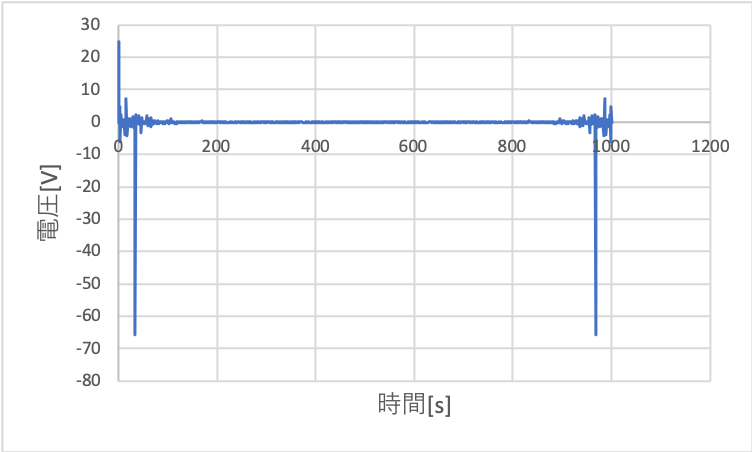
\includegraphics[width=0.8\linewidth]{fig25.png}
 \end{center}
 \caption{330Hz音叉のFFT}
 \label{fig:25}
\end{figure}

\begin{figure}[htbp]
 \begin{center}
  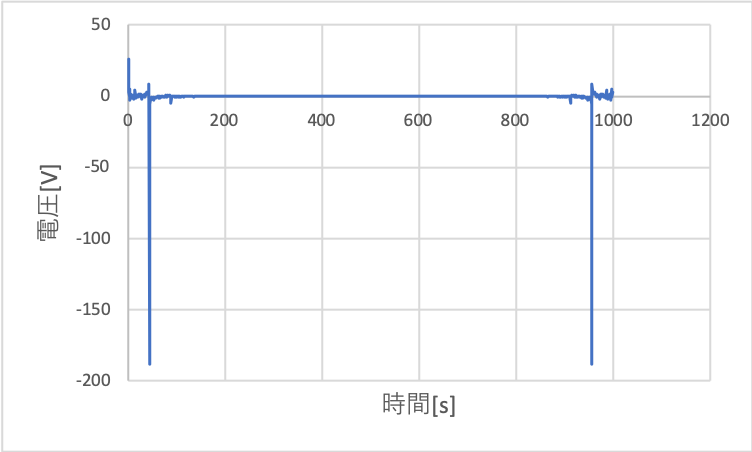
\includegraphics[width=0.8\linewidth]{fig27.png}
 \end{center}
 \caption{440Hz音叉のFFT}
 \label{fig:27}
\end{figure}
\newpage
%============================================================
\subsection{Discussion}
\noindent
\textbf{Task 4.1} \\
まず今回の実験においてのフーリエ変換の式は以下のように与えられる.
\begin{equation}
    F(w) = \int_{\infty}^{\infty}f(t)e^{-2j{\pi}wt}dt
\end{equation}
このことから今回のFFTの結果は横軸が角周波数wになるのではなくサンプリング周波数fになることが読み取れる.
したがって,図\ref{fig:22}においてFFTした結果時間領域[s]の余弦波が周波数[Hz]領域の関数に変換されたと考えられ,3番目のパワースペクトルのグラフにいて262Hz付近の値が大きいことは時間領域における信号が262Hzの周波数を多く含む振動をしていたことを意味するが,実際に今回は262Hzの余弦波をフーリエ変換したので正しく結果が表示されていると考えられる.

また真ん中の虚部の表示においては$10^{-11}$オーダーでの値を示しているのでこれはほぼゼロとみなせる.一方で実部の値は他の値に比べて十分に大きな値を取っていることがわかる.
この原因を考察する.
まず,今回の実験でフーリエ変換の定義域を[0,1-0.001]としいる.この定義域においてフーリエ変換で積分を行うと正弦波と余弦波の積の積分値が0となるため周波数領域でのF(w)が虚部を含まない関数となったことが考えられる.
同様の理由で図\ref{fig:23}の実部において値がほぼ0となっていることにも説明がつく.

さらに今回の時間tはOctaveでt = [1:0.001:1]と定義されているので,1秒間に1000点のサンプルを取ることと同値であると考えられるため今回のサンプリング周波数は1000[Hz]と予想できる.
またFFTの結果が横軸が500のところで折り返しの関係になっている理由としては,まずフーリエ変換においては周波数はサンプリング定理よりF(w)はサンプリング周波数の周期で繰り返されていると予想できる.
つまり周波数領域においてサンプリング周波数をfとすれ[-f/2,f/2]の繰り返しでF(w)が繰り返されていると解釈できる.
今回実験の結果で表示されているのは[0,f]となっている.したがって結果がf/2において線対称になっていることに対して説明がつく.

\noindent
\textbf{Task 4.2} \\
測定において時間領域の信号データは一定の周期で振動していることが確認できるので測定に際して大きなはノイズは発生しなかったと考えられる.
測定はサンプリング周波数10kHz,サンプリング数1000点で行なったのでF(w)の繰り返しの周期は1000となり,周波数の軸は1/10に収縮していると考えられる.
実際FFTしたグラフを観察するとそれぞれf = 34, f = 45のところにトゲが位置しているので概ね正しく測定できたと考えられる.
ところでFFTしたグラフは負の値を持っている.これはOctaveでabsコマンドを打ち損じたことが原因だと考えられる.
フーリエ変換は時間領域で与えられた関数がどのような周波数を含んでいるのか調べるのが目的のため結果はパワースペクトルで示すのが正しいと考えられる.
また周波数軸は(サンプリング周波数)/(データ数)伸縮するので時間領域の信号にどのような周波数が含まれているのか厳密に知りたいときはサンプリング周波数に対してデータ数を多取ると周波数領域においてグラブが引き伸ばされ測定しやすくなると考えられる.



%=============================================================
\newpage
\end{document}
